\begin{problem}[习题4.2]
字符a-h出现的频率分布恰好是前8个Fibonacci数, 它们的Huffman编码是什么? 将结果推广到$n$个字符的频率分布恰好是前$n$个Fibonacci数的情形. Fibonacci数的定义为: $F_0=1$, $F_1=1$, $F_n = F_{n-2}+F_{n-1}$ if $n>1$.
\end{problem}
\begin{solution}
\textbf{解:}根据Fibonacci数的定义求可求出的a-h出现的频率分布, 再由Huffman编码算法可得到Huffman编码树. Huffman编码算法执行过程如图\ref{ah}
\begin{figure}[!htb]
\begin{minipage}[b]{.4\textwidth}
\centering
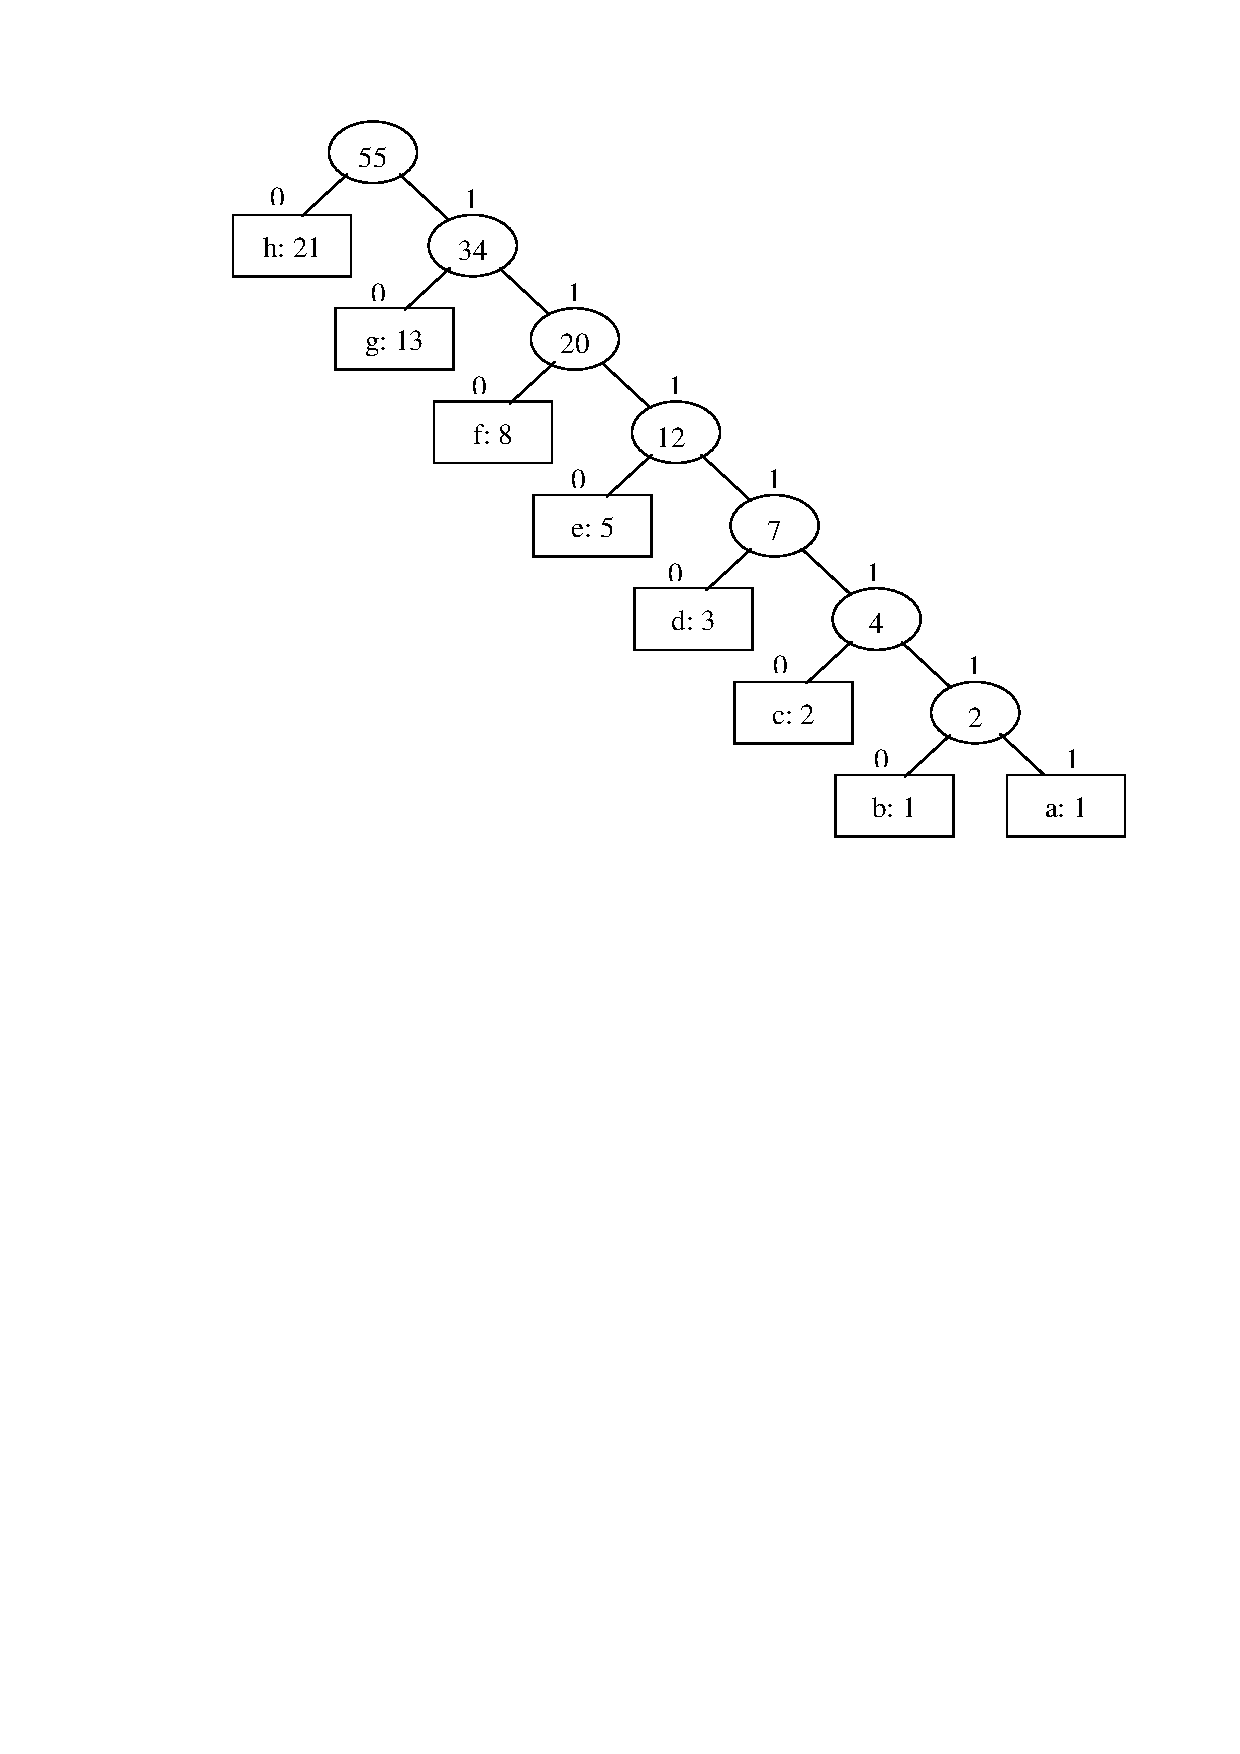
\includegraphics[width=0.8\textwidth]{tree.pdf}
\caption{\label{tree}Huffman编码树}
\end{minipage}%
\begin{minipage}[b]{.6\textwidth}
\centering
\begin{tabular}{l|llllll|l|l|}
\cline{2-9}
1 & \multicolumn{1}{l|}{a:1} & \multicolumn{1}{l|}{b:1} & \multicolumn{1}{l|}{c:2} & \multicolumn{1}{l|}{d:3} & \multicolumn{1}{l|}{e:5} & f:8 & g:13 & h:21 \\
\cline{2-9}
2 & \multicolumn{1}{l|}{c:2} & \multicolumn{2}{l|}{a+b:2} & \multicolumn{1}{l|}{d:3} & \multicolumn{1}{l|}{e:5} & f:8 & g:13 & h:21 \\
\cline{2-9}
3 & \multicolumn{1}{l|}{d:3} & \multicolumn{3}{l|}{(a+b)+c:4} & \multicolumn{1}{l|}{e:5} & f:8 & g:13 & h:21 \\
\cline{2-9}
4 & \multicolumn{1}{l|}{e:5} & \multicolumn{4}{l|}{( (a+b)+c )+d:7} & f:8 & g:13 & h:21 \\
\cline{2-9}
5 & \multicolumn{1}{l|}{f:8} & \multicolumn{5}{l|}{( ( (a+b)+c ) + d) +e:12} & g:13 & h:21 \\
\cline{2-9}
6 & \multicolumn{1}{l|}{g:13} & \multicolumn{6}{l|}{( ( ( (a+b)+c ) + d) +e ) + f:20} & h:21 \\
\cline{2-9}
7 & \multicolumn{1}{l|}{h:21} & \multicolumn{7}{l|}{( ( ( ( (a+b)+c ) + d) +e ) + f ) + g:34} \\
\cline{2-9}
8 & \multicolumn{8}{l|}{( ( ( ( ( (a+b)+c ) + d) +e ) + f ) + g ) + h:55} \\
\cline{2-9}
\end{tabular}
\caption{\label{ah}Huffman编码算法执行过程}
\end{minipage}
\end{figure}
因此, 可得到a-h的Huffman编码, 如图\ref{tree}所示. 可进一步将结果推广到$n$个字符的频率分布恰好是前$n$个Fibonacci数的情形, 第$i$个数的Huffman编码为
\begin{displaymath}
\left\{ \begin{array}{ll}
\overbrace{1\cdots 1}^{n-1\textrm{个}} & i = 1\\
\underbrace{1\cdots 1}_{n-i\textrm{个}}0 & 0< i \leq n\\
\end{array} \right.
\end{displaymath}
\end{solution}
